\documentclass[11pt,compress,blue4,notheorem]{beamer}
\usepackage[T1]{fontenc}
\usepackage{algorithmic}
\usepackage[normalem]{ulem}

%!TEX root =  matrix-est.tex
%\usepackage{etex} % handle MANY packages

% comment this out for the final version, or add the final option:
%\usepackage[notcite,notref]{showkeys}


\usepackage{amsmath,amsbsy,amsfonts,amssymb,amsthm,color,dsfont,mleftright,nccmath}
\usepackage{url}
\usepackage{dsfont} % double stroke font

%%%%%%%%%%%%%%%%%%%%%%%%%%%%%%%%
% PACKAGES
%%%%%%%%%%%%%%%%%%%%%%%%%%%%%%%%
\setlength{\marginparwidth}{25mm}
%\usepackage[textsize=tiny]{todonotes}
\usepackage[disable]{todonotes}
\newcommand{\todoc}[2][]{\todo[color=red!20!white,#1]{Cs: #2}}
\newcommand{\todod}[2][]{\todo[color=blue!20!white,#1]{D: #2}}
\newcommand{\todoa}[2][]{\todo[color=green!20!white,#1]{A: #2}}

\newcommand{\hide}[1]{}

% turn off previously defined macros as we want to use ntheorem (jmlr foolishly defines these)
\if0
\let\proof\relax
\let\endproof\relax
\let\theorem\relax
\let\endtheorem\relax
\let\proposition\relax
\let\endproposition\relax
\let\lemma\relax
\let\endlemma\relax
\let\corollary\relax
\let\endcorollary\relax
\let\example\relax
\let\endexample\relax
\let\remark\relax
\let\endremark\relax
\let\definition\relax
\let\enddefinition\relax
\fi
%\usepackage[amsmath,standard,thmmarks]{ntheorem} % ntheorem makes cleveref work properly 
\newtheorem{lemma}{Lemma}
\newtheorem{claim}{Claim}
\newtheorem{proposition}{Proposition}
\newtheorem{theorem}{Theorem}
\newtheorem{corollary}{Corollary}

\usepackage{latexsym}
%\usepackage{times}
\usepackage{mathtools}
\usepackage{enumerate}
\usepackage[ruled]{algorithm}
\usepackage{algorithmic}
\usepackage{hyperref}
\hypersetup{
    bookmarks=true,         % show bookmarks bar?
    unicode=false,          % non-Latin characters in Acrobat's bookmarks
    pdftoolbar=true,        % show Acrobat's toolbar?
    pdfmenubar=true,        % show Acrobat's menu?
    pdffitwindow=false,     % window fit to page when opened
    pdfstartview={FitH},    % fits the width of the page to the window
    pdftitle={My title},    % title
    pdfauthor={Author},     % author
    pdfsubject={Subject},   % subject of the document
    pdfcreator={Creator},   % creator of the document
    pdfproducer={Producer}, % producer of the document
    pdfkeywords={keyword1} {key2} {key3}, % list of keywords
    pdfnewwindow=true,      % links in new window
    colorlinks=true,       % false: boxed links; true: colored links
    linkcolor=red,          % color of internal links (change box color with linkbordercolor)
    citecolor=blue,        % color of links to bibliography
    filecolor=magenta,      % color of file links
    urlcolor=black          % color of external links
}
%\usepackage[standard]{ntheorem}
%\usepackage{times}
\usepackage[numbers,sort&compress]{natbib}
\usepackage{enumitem}
\usepackage{bibunits}


%\setlist{nolistsep}

%%%%%%%%%%%%%%%%%%%%%%%%%%%%%%%%
% THEOREMS
%%%%%%%%%%%%%%%%%%%%%%%%%%%%%%%%
\if0
\newtheorem{lemma}{Lemma}
\newtheorem{claim}{Claim}
\newtheorem{proposition}{Proposition}
\newtheorem{theorem}{Theorem}
\newtheorem{corollary}{Corollary}
\theoremstyle{remark}
\newtheorem{remark}{Remark}
\theoremstyle{definition}
\newtheorem{definition}{Definition}
\newtheorem{condition}{Condition}
\newtheorem{example}{Example}
\newtheorem{problem}{Problem}
\fi
\usepackage[capitalize]{cleveref}
\usepackage{fullpage}

%%%%%%%%%%%%%%%%%%%%%%%%%%%%%%%%
% MACROS
%%%%%%%%%%%%%%%%%%%%%%%%%%%%%%%%

\def\ddefloop#1{\ifx\ddefloop#1\else\ddef{#1}\expandafter\ddefloop\fi}

% \bA, \bB, ...
\def\ddef#1{\expandafter\def\csname b#1\endcsname{\ensuremath{\mathbf{#1}}}}
\ddefloop ABCDEFGHIJKLMNOPQRSTUVWXYZ\ddefloop

% \bbA, \bbB, ...
\def\ddef#1{\expandafter\def\csname bb#1\endcsname{\ensuremath{\mathbb{#1}}}}
\ddefloop ABCDEFGHIJKLMNOPQRSTUVWXYZ\ddefloop

% \cA, \cB, ...
\def\ddef#1{\expandafter\def\csname c#1\endcsname{\ensuremath{\mathcal{#1}}}}
\ddefloop ABCDEFGHIJKLMNOPQRSTUVWXYZ\ddefloop

% \vA, \vB, ..., \va, \vb, ...
\def\ddef#1{\expandafter\def\csname v#1\endcsname{\ensuremath{\boldsymbol{#1}}}}
\ddefloop ABCDEFGHIJKLMNOPQRSTUVWXYZabcdefghijklmnopqrstuvwxyz\ddefloop

% \valpha, \vbeta, ...,  \vGamma, \vDelta, ...,
\def\ddef#1{\expandafter\def\csname v#1\endcsname{\ensuremath{\boldsymbol{\csname #1\endcsname}}}}
\ddefloop {alpha}{beta}{gamma}{delta}{epsilon}{varepsilon}{zeta}{eta}{theta}{vartheta}{iota}{kappa}{lambda}{mu}{nu}{xi}{pi}{varpi}{rho}{varrho}{sigma}{varsigma}{tau}{upsilon}{phi}{varphi}{chi}{psi}{omega}{Gamma}{Delta}{Theta}{Lambda}{Xi}{Pi}{Sigma}{varSigma}{Upsilon}{Phi}{Psi}{Omega}\ddefloop

\newcommand\Sig{\ensuremath{\varSigma}}
\newcommand\veps{\ensuremath{\varepsilon}}
\newcommand\eps{\ensuremath{\epsilon}}

\renewcommand\t{{\ensuremath{\scriptscriptstyle{\top}}}}

\DeclareMathOperator{\tr}{tr}
\DeclareMathOperator{\diag}{diag}
\DeclareMathOperator{\Diag}{Diag}
\DeclareMathOperator{\rank}{rank}
\DeclareMathOperator{\sign}{sign}
\DeclareMathOperator{\supp}{supp}
\DeclareMathOperator{\vol}{vol}

\DeclareMathOperator{\var}{var}
\DeclareMathOperator{\Var}{Var}

\DeclareMathOperator{\Bd}{bd}
\DeclareMathOperator{\Cl}{cl}
\DeclareMathOperator{\Conv}{conv}
\DeclareMathOperator{\Int}{int}
\DeclareMathOperator{\Null}{ker}
\DeclareMathOperator{\Span}{span}
\DeclareMathOperator{\Range}{ran}

\DeclareMathOperator*{\argmin}{arg\,min}
\DeclareMathOperator*{\argmax}{arg\,max}

\newcommand\wt{\ensuremath{\widetilde}}
\newcommand\wh{\ensuremath{\widehat}}
\renewcommand\v{\ensuremath{\boldsymbol}}

\newcommand\comment[1]{{\color{blue}\{\textbf{Comment}: #1\}}}

\newcommand\parens[1]{(#1)}
\newcommand\norm[1]{\|#1\|}
\newcommand\braces[1]{\{#1\}}
\newcommand\brackets[1]{[#1]}
\newcommand\ceil[1]{\lceil#1\rceil}
\newcommand\abs[1]{|#1|}
\newcommand\ind[1]{\ensuremath{\mathds{1}\{#1\}}}
\newcommand\dotp[1]{\langle #1 \rangle}

\newcommand\Parens[1]{\left(#1\right)}
\newcommand\Norm[1]{\left\|#1\right\|}
\newcommand\Braces[1]{\left\{#1\right\}}
\newcommand\Brackets[1]{\left[#1\right]}
\newcommand\Ceil[1]{\left\lceil#1\right\rceil}
\newcommand\Floor[1]{\left\lfloor#1\right\rfloor}
\newcommand\Abs[1]{\left|#1\right|}
\newcommand\Ind[1]{\ensuremath{\mathds{1}\left\{#1\right\}}}
\newcommand\Dotp[1]{\left\langle #1 \right\rangle}

\newcommand\pimin{\ensuremath{\pi_{\star}}}
\newcommand\gap{\ensuremath{\gamma_{\star}}}
\newcommand\slem{\ensuremath{\lambda_{\star}}}

\newcommand\hatpimin{\ensuremath{\hat\pi_{\star}}}
\newcommand\hatgap{\ensuremath{\hat\gamma_{\star}}}

\newcommand\Geom{\ensuremath{\operatorname{Geom}}}
\newcommand\Sym{\ensuremath{\operatorname{Sym}}}
\newcommand\errm{\ensuremath{\v{\cE}_{\vM}}}
\newcommand\errp{\ensuremath{\v{\cE}_{\vpi}}}
\newcommand\errP{\ensuremath{\v{\cE}_{\vP}}}
\newcommand\errpil{\ensuremath{\v{\cE}_{\vpi,1}}}
\newcommand\errpir{\ensuremath{\v{\cE}_{\vpi,2}}}
\newcommand\tv{\ensuremath{\operatorname{tv}}}
\newcommand\tmix{\ensuremath{t_{\operatorname{mix}}}}
\newcommand\trelax{\ensuremath{t_{\operatorname{relax}}}}
\newcommand\avg{\ensuremath{\operatorname{avg}}}
\newcommand{\iset}[1]{[#1]}
\newcommand{\opencloseint}[1]{\ensuremath{(#1]}}

\newcommand{\Dvpi}{\Diag(\vpi)}
\newcommand{\Dvpit}{\Diag(\vpi^{(t)})}

\newcommand{\EE}[1]{\bbE\left(#1\right)}

\newcommand\giAh{\ensuremath{\widehat{\boldsymbol{A}}^{\raisebox{-2.9pt}{$\scriptstyle\#$}}}}
\newcommand\giA{\ensuremath{\boldsymbol{A}^{\raisebox{-0pt}{$\scriptstyle\#$}}}}
\newcommand{\defeq}{:=}

\newcommand\emptail{\ensuremath{\tau_{n,\delta}}}



\setbeamertemplate{navigation symbols}{}
\setbeamertemplate{footline}{\hfill\insertframenumber\hspace{1mm}\vspace{1mm}}

\definecolor{boldgreen}{rgb}{0.2,0.6,0.2}
\definecolor{darkgreen}{rgb}{0.1,0.4,0.1}
\definecolor{darkblue}{rgb}{0,0,0.7}
\definecolor{firebrick}{rgb}{0.7,0.13,0.13}
\definecolor{britishracinggreen}{rgb}{0.0, 0.26, 0.15}
\newcommand{\RED}[1]{\textcolor{red}{#1}}
\newcommand{\GREEN}[1]{\textcolor{boldgreen}{#1}}
\newcommand{\GRAY}[1]{\textcolor{gray}{#1}}
\newcommand{\LIGHTGRAY}[1]{\textcolor{lightgray}{#1}}
\newcommand{\BLUE}[1]{\textcolor{blue}{#1}}
\newcommand{\FIREBRICK}[1]{\textcolor{firebrick}{#1}}

\newcommand\fns\footnotesize

\newcommand\tv{\ensuremath{\operatorname{tv}}}
\newcommand\tmix{\ensuremath{t_{\operatorname{mix}}}}
\newcommand\tmixhat{\ensuremath{\hat{t}_{\operatorname{mix}}}}
\newcommand\trelax{\ensuremath{t_{\operatorname{relax}}}}
\newcommand\pimin{\ensuremath{\pi_{\star}}}
\newcommand\gap{\ensuremath{\gamma_{\star}}}
\newcommand\hatgap{\ensuremath{\hat{\gamma}_{\star}}}
\newcommand\slem{\ensuremath{\lambda_{\star}}}

\newcommand\states{\ensuremath{\mathcal{X}}}

\AtBeginSection[]
{\begin{frame}<beamer>
\begin{center}
{\Large \thesection. \ \insertsection}
\end{center}
\end{frame}}
\setbeamertemplate{section in toc}[sections numbered]

\title{Confidence intervals for the mixing time \\ of a reversible
Markov chain \\ from a single sample path}
\author{%
  Daniel Hsu$^\dag$ \and
  Aryeh Kontorovich$^\sharp$ \and
  Csaba Szepesv\'ari$^\star$%
}
\institute{%
  $^\dag$Columbia University,
  $^\sharp$Ben-Gurion University,
  $^\star$University of Alberta
}
\date{}

\begin{document}

\begin{frame}
\titlepage

\end{frame}

%-------------------------------------------------------------------------------
%
%\begin{frame}
%\frametitle{Outline}
%\tableofcontents[hideallsubsections]
%\end{frame}

%-------------------------------------------------------------------------------

\begin{frame}
  \frametitle{Problem}

  \begin{itemize}
    \item
      Irreducible, aperiodic, time-homogeneous Markov chain
      \[
        X_1 \ \to \ X_2 \ \to \ X_3 \ \to \ \dotsb
      \]

    \item<2->
      There is a unique \GREEN{stationary distribution} $\pi$ with
      \[
        \lim_{t\to\infty}
        \cL(X_t \mid X_1=x) \ = \ \pi
        \,,
        \quad \text{for all $x \in \states$}
        \,.
      \]

    \item<3->
      The \GREEN{mixing time} $\tmix$ is the earliest time $t$ with
      \[
        \sup_{x \in \states}
        \norm{\cL(X_t \mid X_1=x) - \pi}_{\tv}
        \ \leq \
        1/4
        \,.
      \]

  \end{itemize}

  \onslide<4->
  \textbf{Problem}:

  \medskip
  \begin{overprint}
    \onslide<4>
    \begin{center}
      Determine (confidently) if $t\geq\tmix$ after seeing $X_1,X_2,\dotsc,X_t$.
    \end{center}
    \onslide<5>
    \begin{center}
      Given $\delta \in (0,1)$, determine non-trivial $I_t \subseteq
      [0,\infty]$ from $X_{1:t}$ with
      \[
        \P(\tmix \in I_t) \ \geq \ 1-\delta
        \,.
      \]
    \end{center}
  \end{overprint}

\end{frame}

%-------------------------------------------------------------------------------

\begin{frame}
  \frametitle{Some motivation from machine learning and statistics}

  \textbf{Chernoff bounds for Markov chains $X_1\to X_2\to\dotsb$}:
  \\
  for suitably well-behaved $f \colon \states \to \bbR$,
  with probability at least $1-\delta$,
  \[
    \Abs{
      \frac1t\sum_{i=1}^t f(X_i)
      -
      \E_\pi f
    }
    \ \leq \
    \underbrace{
      \tilde O\Parens{
        \sqrt{
          \frac{\tmix \log(1/\delta)}{t}
        }
      }
    }_{\text{deviation bound}}
    \,.
  \]
  \FIREBRICK{Bound depends on $\tmix$, which may be unknown \emph{a
  priori}}.

  \onslide<2->
  \bigskip
  \textbf{Examples}:
  \begin{description}
    \item[Bayesian inference]
      \underline{Posterior means \& variances} via MCMC

    \item[Reinforcement learning]
      \underline{Mean action rewards} in an MDP

    \item[Supervised learning]
      \underline{Error rates of hypotheses} from non-iid data

  \end{description}

  \onslide<3->
  \begin{center}
    \BLUE{%
      Need observable deviation bounds.
    }
  \end{center}

\end{frame}

%-------------------------------------------------------------------------------

\begin{frame}
  \frametitle{Observable deviation bounds from mixing time bounds?}

  Suppose an estimator $\tmixhat = \tmixhat(X_{1:t})$ of
  $\tmix$ satisfies:
  \[
    \P(\tmix \leq \tmixhat + \veps_t)
    \ \geq \
    1-\delta
    \,.
  \]
  \onslide<2->
  Then with probability at least $1-2\delta$,
  \[
    \Abs{
      \frac1t\sum_{i=1}^t f(X_i)
      -
      \E_\pi f
    }
    \ \leq \
    \tilde O\Parens{
      \sqrt{
        \frac{\parens{\tmixhat + \veps_t} \log(1/\delta)}{t}
      }
    }
    \,.
  \]

  \onslide<3->
  But $\tmixhat$ is computed from $X_{1:t}$, so
  \FIREBRICK{$\veps_t$ may also depend on $\tmix$}.

  \onslide<4->
  \begin{center}
    \FIREBRICK{%
      Deviation bounds for point estimators are insufficient.%
    }
    \\
    \BLUE{%
      Need \emph{observable confidence intervals} for $\tmix$.%
    }
  \end{center}

\end{frame}

%-------------------------------------------------------------------------------

\begin{frame}
  \frametitle{What we do}

  \begin{enumerate}
    \item<2->
      Shift focus to \GREEN{relaxation time} $\trelax$ to enable
      spectral methods.

      \medskip

    \item<3->
      \textbf{Lower/upper bounds} on sample path length for point
      estimation of $\trelax$.

      \medskip

    \item<4->
      \textbf{New algorithm} for constructing confidence intervals for
      $\trelax$.

  \end{enumerate}

\end{frame}

%-------------------------------------------------------------------------------

\begin{frame}
  \frametitle{Relaxation time}

  \begin{itemize}
    \item
      Let $P$ be the \GREEN{transition operator} of the Markov chain,

      and let $\slem$ be its \GREEN{second-largest eigenvalue modulus}

      {\fns(i.e., largest eigenvalue modulus other than $1$)}.

      \medskip

    \item<2->
      \GREEN{Spectral gap}: $\gap := 1-\slem$.

      \GREEN{Relaxation time}: $\trelax := 1/\gap$.

      \[
        \Parens{ \trelax - 1 } \ln 2
        \ \leq \
        \tmix
        \ \leq \
        \trelax \ln \frac4{\pimin}
      \]
      for $\pimin := \min_{x \in \states} \pi(x)$.

      \onslide<3->
      \medskip
      Assumptions on $P$ ensure $\gap, \pimin \in (0,1)$.

  \end{itemize}

  \onslide<4->
  \begin{center}
    \BLUE{%
      \textbf{Spectral approach}: construct CI's for $\gap$ and $\pimin$.
    }
  \end{center}

\end{frame}

%-------------------------------------------------------------------------------

\begin{frame}
  \frametitle{Our results (point estimation)}

  We restrict to \GREEN{reversible Markov chains} on \GREEN{finite
  state spaces}.

  Let $d$ be the (known \emph{a priori}) cardinality of the state
  space $\states$.

  \begin{enumerate}
    \item<2->
      {\fns\textbf{Lower bound}:} \\
      To estimate $\gap$ within a constant multiplicative factor,
      \mbox{every algorithm} needs (w.p.~$1/4$) sample path of
      length
      \[
        \geq \
        \Omega\Parens{
          \frac{d \log d}{\gap} + \frac1{\pimin}
        }
        \,.
      \]

    \item<3->
      {\fns\textbf{Upper bound}:} \\
      Simple algorithm estimates $\gap$ and $\pimin$ within a constant
      multiplicative factor (w.h.p.) with sample path of length
      \begin{align*}
        \wt O\Parens{ \frac{\log d}{\pimin\gap^3} }
        & \quad
        \text{(for $\gap$)}
        \,,
        &
        \wt O\Parens{ \frac{\log d}{\pimin\gap} }
        & \quad
        \text{(for $\pimin$)}
        \,.
      \end{align*}

  \end{enumerate}

  \onslide<4->
  \begin{center}
    \FIREBRICK{%
      But point estimator $\not\Rightarrow$ observable
      confidence interval.
    }
  \end{center}

\end{frame}

%-------------------------------------------------------------------------------

\begin{frame}
  \frametitle{Our results (confidence intervals)}

  \begin{enumerate}
    \item[3.]
      \textbf{New algorithm}:
      Given $\delta \in (0,1)$ and $X_{1:t}$ as input, constructs
      intervals $I_t^{\gap}$ and $I_t^{\pimin}$ such that
      \[
        \P\Parens{
          \gap \in I_t^{\gap}
        }
        \ \geq \ 1-\delta
        \quad
        \text{and}
        \quad
        \P\Parens{
          \pimin \in I_t^{\pimin}
        }
        \ \geq \ 1-\delta
        \,.
      \]

      Widths of intervals converge a.s.~to zero at
      $\sqrt{\frac{\log\log t}{t}}$ rate.

      \medskip

    \item[4.]<2->
      \textbf{Hybrid approach}:
      Use new algorithm to turn error bounds for point estimators into
      observable CI's.

      {\fns(This improves asymptotic rate for $\pimin$ interval.)}

  \end{enumerate}

\end{frame}

%-------------------------------------------------------------------------------

\begin{frame}
  \frametitle{Plug-in estimator}

  \begin{itemize}
    \item<2->
      Reversibility grants the symmetry of
      \[
        M
        \ := \
        \diag(\pi) P
        \ = \
        \Braces{ \P_{X_1 \sim \pi}(X_1=x,X_2=x') }_{x,x'\in\states}
      \]
      {\fns(doublet state probabilities in stationary chain)}.

      \smallskip

    \item<3->
      Moreover, eigenvalues of
      \[
        L
        \ := \
        \diag(\pi)^{-1/2} M \diag(\pi)^{-1/2}
      \]
      are real, and satisfy
      \begin{gather*}
        1
        \ = \ \lambda_1 \ > \ \lambda_2 \ \geq \ \dotsb \ \geq \
        \lambda_d \ > \ -1
        \,,
        \\
        \gap
        \ = \ 1 - \max\braces{ \lambda_2, \abs{\lambda_d} }
        \,.
      \end{gather*}

      \smallskip

    \item<4->
      \textbf{Plug-in estimator}:
      estimate $\pi$ and $M$ from $X_{1:t}$ (using empirical
      frequencies), then plug-in to formula for $\gap$.

  \end{itemize}

\end{frame}

%-------------------------------------------------------------------------------

\begin{frame}
  \frametitle{Chicken-and-egg problem}

  (Matrix) Chernoff bound {\fns(for Markov chains)} gives error bounds
  for estimates of $\pi$ and $M$ (and ultimately of $L$ and $\gap$):
  e.g., w.h.p.,
  \[
    \abs{\hatgap-\gap}
    \ \leq \
    \norm{\wh L - L}
    \ \leq \
    O\Parens{
      \sqrt{\frac{\log(d)\log(t/\pimin)}{\gap\pimin t}}
    }
    \,.
  \]
  \onslide<2->
  This has \FIREBRICK{\emph{inverse} dependence} on $\gap$.

  \onslide<3->
  \begin{center}
    \FIREBRICK{%
      Can't ``solve the bound'' for $\gap$
    }

    {\fns(\emph{c.f.} ``empirical Bernstein'' inequalities)}.

    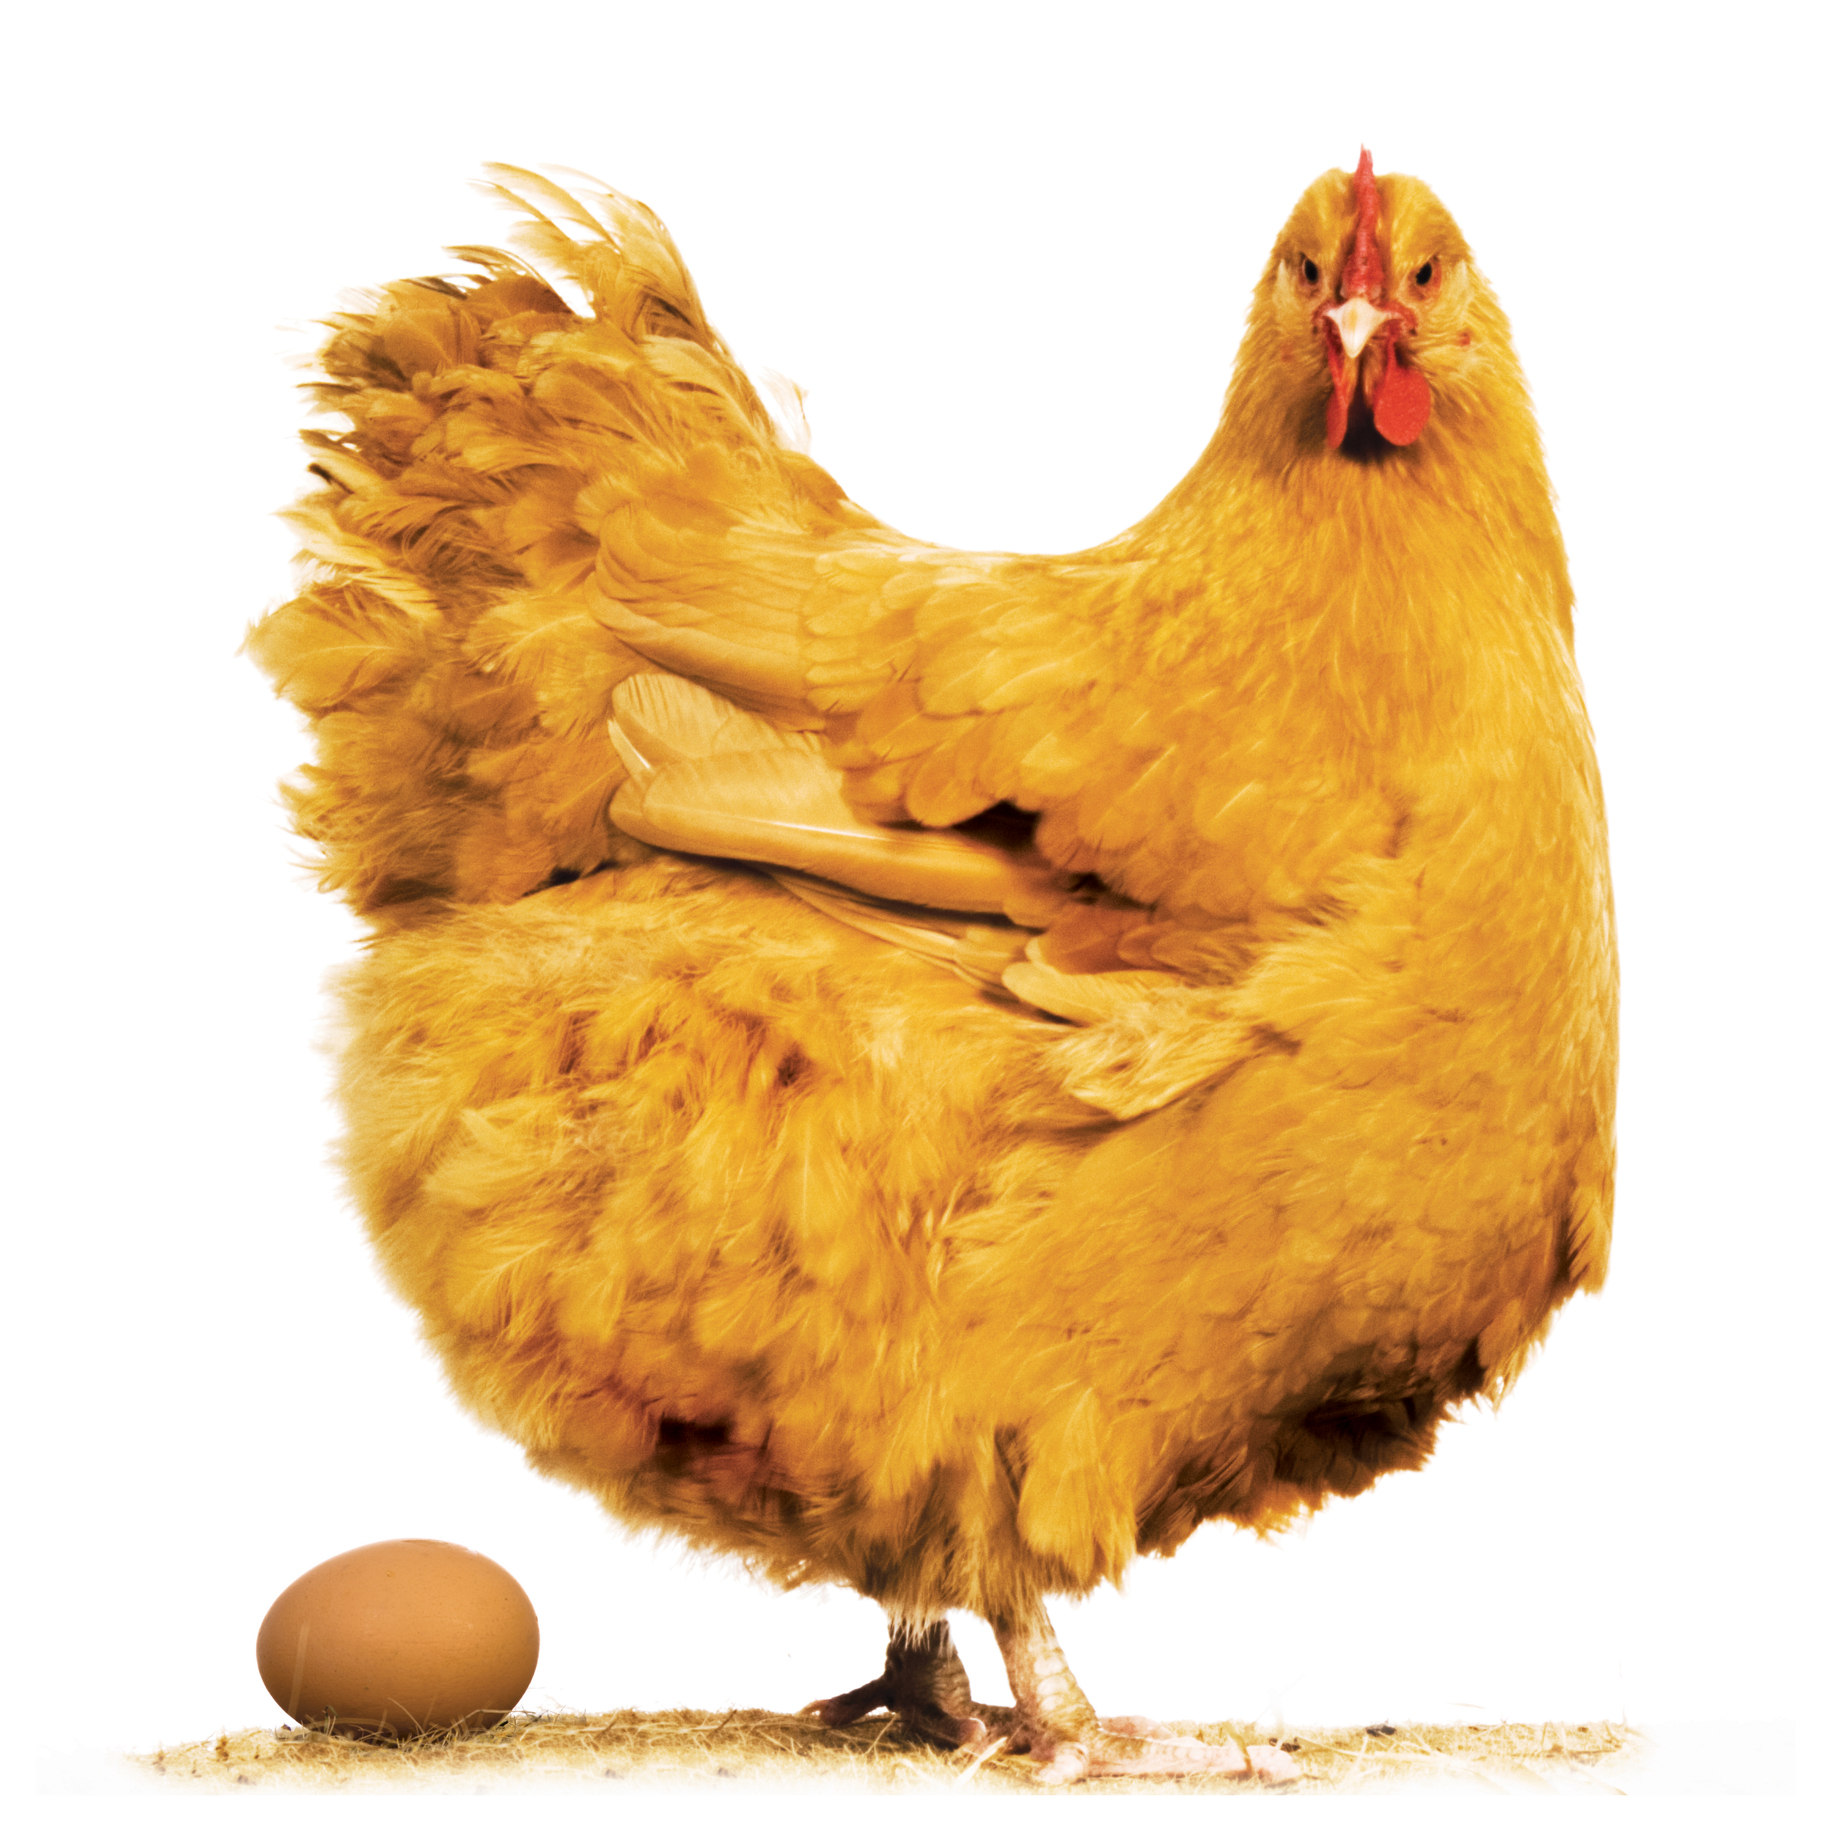
\includegraphics[height=1.5in]{chicken-and-egg.jpg}
  \end{center}

\end{frame}

%-------------------------------------------------------------------------------

\begin{frame}
  \frametitle{Direct estimation of $P$}

  \textbf{Alternative}: directly estimate $P$ from $X_{1:t}$.

  \begin{itemize}
    \item<2->
      \textbf{Key advantage}: observable confidence intervals for $P$
      via ``empirical Bernstein'' inequality for martingales.

  \end{itemize}

  \onslide<3->
  \textbf{Two problems}:
  \begin{enumerate}
    \item<4->
      Without appealing to symmetry structure via $L$, can argue
      \[
        \norm{\wh{P} - P} \ \leq \ \veps
        \quad\Longrightarrow\quad
        \abs{\hatgap - \gap} \ \leq \ O(\veps^{1/(2d)})
        \,,
      \]
      but this implies \FIREBRICK{exponential slow-down in rate}.

      \medskip

    \item<5->
      Appealing to symmetry structure via $L$, get bounds that depend
      on $\pi$, which is unknown.

  \end{enumerate}

  \onslide<6->
  \begin{center}
    \BLUE{%
      \textbf{Our approach}: \\
      Directly estimate $P$, and \emph{indirectly} estimate $\pi$ via
      $\wh P$.
    }
  \end{center}

\end{frame}

%-------------------------------------------------------------------------------

\begin{frame}
  \frametitle{Indirect estimation of $\pi$}

  \begin{enumerate}
    \item
      We ensure that $\wh P$ is transition operator for an ergodic chain
      {\fns(easy via Laplace smoothing)}.

      \medskip

    \item<2->
      \textbf{Key step}: estimate $\pi$ via $\wh P$ via \GREEN{group
      inverse} $\wh A^\#$ of $I - \wh P$.

      \medskip

      \begin{itemize}
        \item<3->
          $\wh A^\#$ contains ``virtually everything that one would want
          to know about the chain'' [with transition operator $\wh P$]
          {\fns(Meyer, 1975)}.

          \medskip

        \item<4->
          Reveals unique stationary distribution $\hat\pi$ w.r.t.~$\wh P$.

          \BLUE{This is our indirect estimate of $\pi$}.

          \medskip

        \item<5->
          Tells us how to bound $\norm{\hat\pi-\pi}_\infty$ in terms of
          $\norm{\wh P - P}$.

          \BLUE{Hence, from this, we construct a confidence interval
          for $\pi$.}

      \end{itemize}

%    \item
%      Use \GREEN{perturbation theory for eigenvalues of symmetric
%      operators} to get \BLUE{confidence interval for $\gap$ in terms
%      of confidence intervals for $P$ and $\pi$}.
%
  \end{enumerate}

\end{frame}

%-------------------------------------------------------------------------------

\begin{frame}
  \frametitle{Overall algorithm (outline)}

  \begin{enumerate}
    \item
      Form empirical estimate and confidence intervals for $P$

      {\fns(exploit Markov property \& ``empirical Bernstein''-type bounds)}.

      \medskip

    \item
      Form estimate and confidence intervals for $\pi$

      {\fns(via group inverse of $I - \wh P$)}.

      \medskip

    \item
      Form estimate and confidence interval for $\gap$

      {\fns(via confidence intervals for $\pi$ and $P$, \& eigenvalue perturbation theory)}.

  \end{enumerate}
\end{frame}

%-------------------------------------------------------------------------------

\begin{frame}
  \frametitle{Recap and future work}

  \begin{itemize}
    \item
      We resolve ``chicken-and-egg'' problem of observable
      confidence intervals for mixing time from a single sample path.

    \item<2->
      Strongly exploit Markov property and ergodicity in confidence
      intervals for $P$ and $\pi$.

    \item<3->
      \textbf{Problem \#1}:
      \textcolor{britishracinggreen}{%
        close gap between lower and upper bounds on sample path length
        (for point estimation).%
      }

    \item<4->
      \textbf{Problem \#2}:
      \textcolor{britishracinggreen}{%
        overcome computational bottlenecks from matrix operations.%
      }

    \item<5->
      \textbf{Problem \#3}:
      \textcolor{boldgreen}{%
        handle large/continuous state spaces under suitable
        assumptions.%
      }

  \end{itemize}

\end{frame}

%-------------------------------------------------------------------------------

\begin{frame}
  \begin{center}
    \Huge
    Thanks!
  \end{center}
\end{frame}

%-------------------------------------------------------------------------------

\end{document}

